\documentclass{article}\usepackage[]{graphicx}\usepackage[]{color}
%% maxwidth is the original width if it is less than linewidth
%% otherwise use linewidth (to make sure the graphics do not exceed the margin)
\makeatletter
\def\maxwidth{ %
  \ifdim\Gin@nat@width>\linewidth
    \linewidth
  \else
    \Gin@nat@width
  \fi
}
\makeatother

\definecolor{fgcolor}{rgb}{0.345, 0.345, 0.345}
\newcommand{\hlnum}[1]{\textcolor[rgb]{0.686,0.059,0.569}{#1}}%
\newcommand{\hlstr}[1]{\textcolor[rgb]{0.192,0.494,0.8}{#1}}%
\newcommand{\hlcom}[1]{\textcolor[rgb]{0.678,0.584,0.686}{\textit{#1}}}%
\newcommand{\hlopt}[1]{\textcolor[rgb]{0,0,0}{#1}}%
\newcommand{\hlstd}[1]{\textcolor[rgb]{0.345,0.345,0.345}{#1}}%
\newcommand{\hlkwa}[1]{\textcolor[rgb]{0.161,0.373,0.58}{\textbf{#1}}}%
\newcommand{\hlkwb}[1]{\textcolor[rgb]{0.69,0.353,0.396}{#1}}%
\newcommand{\hlkwc}[1]{\textcolor[rgb]{0.333,0.667,0.333}{#1}}%
\newcommand{\hlkwd}[1]{\textcolor[rgb]{0.737,0.353,0.396}{\textbf{#1}}}%
\let\hlipl\hlkwb

\usepackage{framed}
\makeatletter
\newenvironment{kframe}{%
 \def\at@end@of@kframe{}%
 \ifinner\ifhmode%
  \def\at@end@of@kframe{\end{minipage}}%
  \begin{minipage}{\columnwidth}%
 \fi\fi%
 \def\FrameCommand##1{\hskip\@totalleftmargin \hskip-\fboxsep
 \colorbox{shadecolor}{##1}\hskip-\fboxsep
     % There is no \\@totalrightmargin, so:
     \hskip-\linewidth \hskip-\@totalleftmargin \hskip\columnwidth}%
 \MakeFramed {\advance\hsize-\width
   \@totalleftmargin\z@ \linewidth\hsize
   \@setminipage}}%
 {\par\unskip\endMakeFramed%
 \at@end@of@kframe}
\makeatother

\definecolor{shadecolor}{rgb}{.97, .97, .97}
\definecolor{messagecolor}{rgb}{0, 0, 0}
\definecolor{warningcolor}{rgb}{1, 0, 1}
\definecolor{errorcolor}{rgb}{1, 0, 0}
\newenvironment{knitrout}{}{} % an empty environment to be redefined in TeX

\usepackage{alltt}[12pt]
\usepackage{Sweave}
\usepackage{float}
\usepackage{graphicx}
\usepackage{tabularx}
\usepackage{siunitx}
\usepackage[margin=2.5cm]{geometry}
\usepackage{pdflscape}
\usepackage{mdframed}
\usepackage{natbib}
\bibliographystyle{..//refs/styles/gcb}
\usepackage[hyphens]{url}
\usepackage[small]{caption}
\setlength{\captionmargin}{30pt}
\setlength{\abovecaptionskip}{0pt}
\setlength{\belowcaptionskip}{10pt}
%\topmargin -2.5cm        
%\oddsidemargin -2.5cm   
%\evensidemargin -2.5cm
\textwidth 16.59cm
\textheight 21.94cm 
%\pagestyle{empty} %comment if want page numbers
\parskip 7.2pt
\renewcommand{\baselinestretch}{2}
\parindent 0pt
\usepackage{lineno}
\linenumbers
\usepackage{setspace}
\doublespacing

\newmdenv[
  topline=true,
  bottomline=true,
  skipabove=\topsep,
  skipbelow=\topsep
]{siderules}

%% R Script


\IfFileExists{upquote.sty}{\usepackage{upquote}}{}
\begin{document}
\noindent \textbf{\Large{Rethinking False Spring Risk}}

\noindent Authors:\\
C. J. Chamberlain $^{1,2}$, B. I. Cook $^{3}$, I. Garcia de Cortazar Atauri $^{4}$ \& E. M. Wolkovich $^{1,2,5}$
\vspace{2ex}\\
\emph{Author affiliations:}\\
$^{1}$Arnold Arboretum of Harvard University, 1300 Centre Street, Boston, Massachusetts, USA; \\
$^{2}$Organismic \& Evolutionary Biology, Harvard University, 26 Oxford Street, Cambridge, Massachusetts, USA; \\
$^{3}$NASA Goddard Institute for Space Studies, New York, New York, USA; \\
$^{4}$French National Institute for Agricultural Research, INRA, US1116 AgroClim, F-84914 Avignon, France\\
$^{5}$Forest \& Conservation Sciences, Faculty of Forestry, University of British Columbia, 2424 Main Mall, Vancouver, BC V6T 1Z4\\
\vspace{2ex}
$^*$Corresponding author: 248.953.0189; cchamberlain@g.harvard.edu\\

\noindent \emph{Keywords:} false spring, phenology, freezing tolerance, climate change, forest communities \\
%\tableofcontents
\emph{Paper type:} Opinion
%\emph{Counts}: Total word count for the main body of the text:  2611; Abstract: 119; 4 figures (all in color). \\

\renewcommand{\thetable}{\arabic{table}}
\renewcommand{\thefigure}{\arabic{figure}}
\renewcommand{\labelitemi}{$-$}
\setkeys{Gin}{width=0.8\textwidth}

%%%%%%%%%%%%%%%%%%%%%%%%%%%%%%%%%%%%%%%%%%%%%%%
% General to do
% Move all figures and their captions to end of manuscript
% Work on transitions throughout. I made note of it many places.
% My comments are usually in [] and I made some edits throughout. You can use the app FileMerge (spotlight search for it) on most Macs to see the changes quickly. 
%%%%%%%%%%%%%%%%%%%%%%%%%%%%%%%%%%%%%%%%%%%%%%%

\newpage
\section*{Abstract} % (239/300)
% Cat: I think we need to rewrite this to better reflect the current draft of the paper. Some of the clauses and sentences in the conclusion section (pasted below) would help I think, but we also probably need some new text to highlight how cool the current paper is (compared to when last we worked on this abstract in earnest). So I started work on this, see what you think, it definitely needs work. 
Temperate plants are at risk of being exposed to late spring freezes. These freeze events---often called false springs---are one of the strongest factors determining temperate plants species range limits and can impose high ecological and economic damage. As climate change may alter the prevalence and severity of false springs, our ability to forecast such events has become more critical. Currently, many false spring studies largely simplify the myriad complexities involved in assessing false spring damage and risks. While these studies have helped greatly advanced the field to date and may provide useful estimates at large scales, studies at the individual to community levels must integrate more complexity for accurate predictions of the level of plant damage from late spring freezes. Here we review current metrics of false spring, and how, when and where plants are most at risk of freeze damage. We highlight how life stage, functional group, species differences in morphology and phenology, and regional climatic differences contribute to the damage potential of false springs. More studies aimed at understanding relationships among species tolerance and avoidance strategies, climatic regimes, and the environmental cue that underlie spring pheneology would improve predictions at all biological levels. An integrated approach to assessing past and future spring freeze damage would provide novel insights into fundamental plant biology, and offer more robust predictions as climate change progresses, which is essential for mitigating the adverse ecological and economic effects of false springs. %(The ultimate intent is to demonstrate how an integrated view of false spring that incorporates these factors would rapidly advance progress in this field.)
% Integrating these complexities could rapidly advance forecasting of false spring events in climate change and ecological studies.

% In this paper we aim to highlight the complexity of factors driving a plant's false spring risk and provide a road map for improved metrics. First, we review the currently used definitions of false spring. Then, combining research from plant physiology, climatology and community ecology, we outline major gaps in current definitions.

% Current metrics for estimating false springs events often require only two pieces of information: an estimate for the start of biological `spring' (i.e., budburst) and whether temperatures below a particular threshold occurred in the following week. Such estimates provide a basic understanding of potential false spring events. However, they inherently assume consistency of damage across functional groups, species, life stages, and regional climates, ignoring that such factors can greatly impact plants' false spring risk. As a result, such indices may lead to inaccurate estimates and predictions, slowing our progress in understanding false spring events and how they may shift with climate change. To produce accurate predictions, researchers need improved methods that can properly evaluate the effects of false springs across diverse species and climate regimes.


% With warm temperatures advancing in the spring but last spring freeze dates advancing at a slower rate, there could be more damaging false spring events in the future, especially in high-risk regions \citep{Gu2008, Inouye2008, Liu2018}. Simple equations for evaluating false spring damage (e.g., Equation \ref{eq:1}) largely simplify the myriad complexities involved in assessing false spring damage and risks. More studies aimed at understanding relationships among species tolerance and avoidance strategies, climatic regimes, and physiological cue interactions with the duration of vegetative risk would improve predictions and ecosystem models that will hopefully replace our current metric. Additionally, research to establish temperature thresholds for damage across functional types and phenophases will help effectively predict false spring risk in the future. An integrated approach to assessing past and future spring freeze damage would provide novel insights into the fundamental plant strategies, and offer more robust predictions as climate change progresses, which is essential for mitigating the adverse ecological and economic effects of false springs.

\section*{Introduction}

Plants from temperate environments time their growth each spring to follow rising temperatures alongside the increasing availability of light and soil resources. During this time, individuals that budburst before the last freeze date are at risk of leaf loss, damaged wood tissue, and slowed canopy development \citep{Gu2008, Hufkens2012}. These damaging late spring freezes are also known as false springs, and are widely documented to result in adverse ecological and economic consequences \citep{Ault2013, Knudson2012}.

Climate change is expected to cause an increase in damage from false spring events due to earlier spring onset and potentially greater fluctuations in temperature in some regions \citep{Inouye2008, Martin2010}. In recent years multiple studies have documented false springs \citep{Augspurger2009, Augspurger2013, Gu2008, Menzel2015} and some have linked these events to climate change \citep{Allstadt2015, Ault2013,  Muffler2016, Vitra2017, Xin2016}. This interest in false springs has led to a growing body of research investigating the effects across ecosystems. Such work builds on decades of work across the fields of ecophysiology, climatology, ecosystem and alpine ecology examining how spring frosts have shaped the life history strategies of diverse species and determine the dynamics of many ecosystems, especially in temperate and boreal systems where frost is a common obstacle to plant growth. While this literature has highlighted the complexity of factors that underlie false springs, many current estimates seek to simplify the process. 

Current metrics for estimating false springs events often require only two pieces of information: an estimate for the start of biological `spring' (i.e., budburst) and whether temperatures below a particular threshold occurred in the following week. Such estimates provide a basic understanding of potential false spring events. However, they inherently assume consistency of damage across functional groups, species, life stages, and regional climates, ignoring that such factors can greatly impact plants' false spring risk. As a result, such indices may lead to inaccurate estimates and predictions, slowing our progress in understanding false spring events and how they may shift with climate change. To produce accurate predictions, researchers need improved methods that can properly evaluate the effects of false springs across diverse species and climate regimes.

In this paper we highlight the complexity of factors driving a plant's false spring risk and provide a road map for improved metrics. We show how freeze temperature thresholds \citep{Lenz2013}, location within a forest or canopy \citep{Augspurger2013}, interspecific variation in avoidance and tolerance strategies \citep{Martin2010, Muffler2016}, and regional effects \citep{Muffler2016} unhinge simple metrics of false spring. We argue that while current simplified metrics have advanced the field and offer further advances at large scales, greater progress can come from new approaches. In particular, approaches that integrate the major factors shaping false spring risk would help accurately determine current false spring damage and improve predictions of spring freeze risk under a changing climate --- while potentially providing novel insights to how plants respond to and are shaped by spring frost. We focus on temperate forests, where much recent and foundational research has been conducted, but our suggestions and findings apply to any ecosystem shaped by spring frosts events. % The ultimate intent is to demonstrate how an integrated view of false spring that incorporates these factors would rapidly advance progress in this field.  


%%%%%%%%%%%%%%%%%%%%%%%%%%%%%%%%%%%%%%%%%%%%%%%%%%%%%%%%%%%
\section*{Defining false springs} 
\subsection*{When are plants vulnerable to frost damage?} 
%%%%%%%%%%%%%%%%%%%%%%%%%%%%%%%%%%%%%%%%%%%%%%%%%%%%%%%%%%%
% Lots of edits here: In trying to address R2 I have aimed for a section that summarizes background info without making too many new assertions. See what you think.
At the level of an individual plant, vulnerability to frost damage varies across tissues and seasonally with plant development. Some tissues are often more or less sensitive to low temperatures. Flower and fruit tissues, are often easily damaged by freezing temperatures \citep{Inouye2000, Augspurger2009,Lenz2013, Caradonna2016}, while wood and bark tissues can survive lower temperatures through various methods \citep{Strimbeck2015}. Similar to wood and bark, leaf and bud tissues can often survive lower temperatures without damage \citep{Charrier2011}. However, for most wood and vegetative tissues, tolerance of low temperatures varies seasonally with the environment through the development of cold hardiness (i.e. freezing tolerance), which allows plants to survive colder winter temperatures through various physiological mechanisms \citep[] [e.g., deep supercooling, increased solute concentration, and an increase in dehydrins and other proteins] {Sakai1987, Strimbeck2015}. 

% Cat: again, see below where I added something, please correct what triggers hardiness! 
Cold hardiness is an essential process for temperate plants to survive cold winters and hard freezes \citep{Vitasse2014}, especially in allowing bud tissue to overwinter without damage. Much cold hardiness research focuses on vegetative and floral buds, especially in the agricultural literature (where much fundamental research has occurred), where buds greatly determine crop success each season. 

% Think about adding a section that incorporates fall dehardening and rehardening?

% Cat: again, see changes, add cites.
The actual temperatures that plants can tolerate varies strongly by species (Figure \ref{fig:temp}) and by a tissue's degree of cold hardiness. During the cold acclimation phase --- which is generally triggered by shorter photoperiods \citep{Welling1997, Howe2003, Charrier2011, Strimbeck2015} and, in some species, cold nights \citep{Heide2005, Charrier2011} --- cold hardiness increases rapidly as temperate plants begin to enter dormancy. Once buds reach the dormancy phase, buds are able to tolerate lower temperates \citep[ to -60$^{\circ}$C in extreme cases,][] {Korner2012}. At maximum cold hardiness vegetative tissues can generally sustain temperatures from -25$^{\circ}$C to -40$^{\circ}$C \citep{Charrier2011,Korner2012,Vitasse2014}, with some species surviving -60$^{\circ}$C or lower without damage. Freezing tolerance diminishes again during the cold deacclimation phase, when metabolism and development start to increase, and plant tissues become especially vulnerable. Once buds begin to swell and deharden, freezing tolerance greatly diminishes and is lowest between budburst to leafout (i.e., around -2 to -3$^{\circ}$C), then generally increases slightly once the leaves fully mature \citep[] [i.e., around -3 to -5$^{\circ}$C] {Lenz2013}. Thus, plants that have initiated budburst but have not fully leafed out are more likely to sustain damage from a false spring than individuals past the leafout phase \citep{Lenz2016}. This timing is also most critical when compared to the fall onset of cold hardiness: as plants generally senesce as they gain cold hardiness, tissue damage during the fall is far less common and less critical \citep{Estiarte2015, Liu2018}.  

Temperate forest plants, therefore, experience elevated risk of frost damage during the spring due both to the stochastic timing of frosts and the rapid decrease in freezing tolerance, which can have important consequences for individual plants all the way up to the ecosystem-level. Freezing temperatures following a warm spell can result in plant damage or even death \citep{Ludlum1968, Mock2007}. It can take 16-38 days for trees to refoliate after a spring freeze \citep{Gu2008, Augspurger2009, Augspurger2013, Menzel2015}, which can detrimentally affect crucial processes such as carbon uptake and nutrient cycling \citep{Hufkens2012, Richardson2013, Klosterman2018}. Additionally, plants will suffer greater long-term effects from the loss of photosynthetic tissue, which could impact multiple years of growth, reproduction, and canopy development \citep{Vitasse2014, Xie2015}.  For these reasons, we focus primarily on spring freeze risk for the vegetative phases, specifically between budburst and leafout, when vegetative tissues are most at risk of damage.

\begin{figure}[H]

{\centering 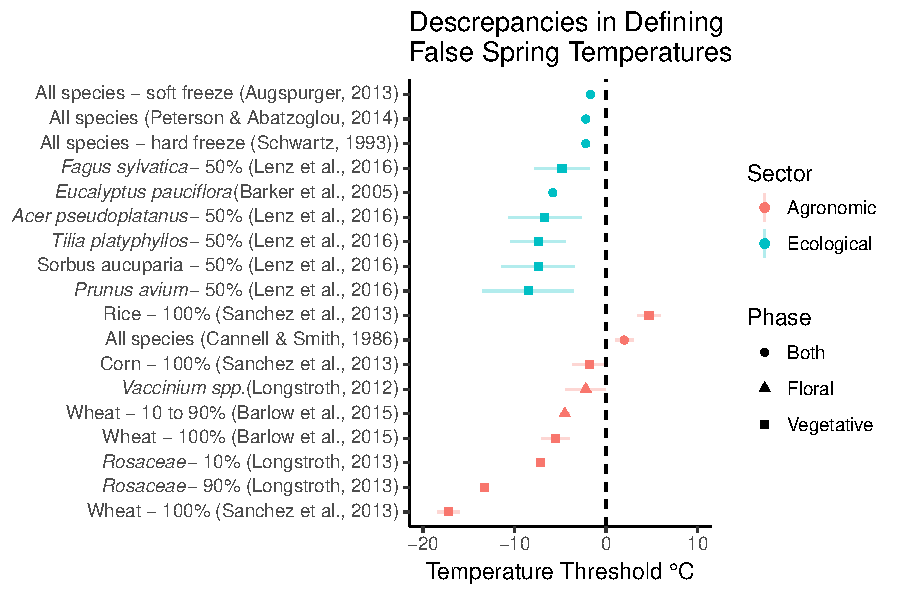
\includegraphics[width=\maxwidth]{figure/temp-1} 

}

\caption[A comparison of damaging spring freezing temperature thresholds across ecological and agronomic studies]{A comparison of damaging spring freezing temperature thresholds across ecological and agronomic studies. Each study is listed on the vertical axis along with the taxonomic group of focus. Next to the species name is the freezing definition used within that study (e.g., 100\% is 100\% whole plant lethality). Each point is the best estimate recorded for the temperature threshold with standard deviation if indicated in the study.}\label{fig:temp}
\end{figure}




\subsection*{Current metrics of false spring}
Currently researchers use several methods to define a false spring. A common definition is fundamentally empirical and describes a false spring as having two phases: rapid vegetative growth prior to a freeze and a post-freeze setback \citep{Gu2008}. However, as data on tissue damage is often lacking most definitions do not require it. Other definitions focus on temperatures in the spring that are specific to certain regions \citep[e.g., in][false spring for the Midwestern United States is defined as a warmer than average March, a freezing April, and enough growing degree days between budburst and the last freeze date]{Augspurger2013}. A widely used definition integrates a mathematical equation to quantify a false spring event. This equation, known as a False Spring Index (FSI), signifies the likelihood of damage to occur from a late spring freeze. Currently, FSI is evaluated annually by the day of budburst and the day of last spring freeze \citep[often calculated at -2.2$^{\circ}$C,][]{Schwartz1993} through the simple equation \citep{Marino2011}:
\begin{equation} \label{eq:1}
FSI = \text{Day of Year} (Last Spring Freeze) - \text{Day of Year} (Budburst)
\end{equation}
Negative values indicate no-risk situations, whereas a damaging FSI is currently defined to be seven or more days between budburst and the last freeze date (Equation \ref{eq:1}) \citep{Peterson2014}. This index builds off our fundamental understanding that cold hardiness is low following budburst (i.e., the seven-day threshold attempts to capture that leaf tissue is at high risk of damage from frost in the period after budburst but before full leafout), and, by requiring only data on budburst and temperatures, this index can estimate where and when false springs occurred (or will occur) without any data on tissue damage. 

\subsection*{Measuring false spring in one temperate plant community}
% Cat: I think we probably should do more here to address R3's request that we discuss the difficulties of defining one date for spring onset but WHY you might want to do that... I tried to weave this throughout, see what you think. 
To demonstrate how the FSI definition works---and is often used---we applied it to data from the Harvard Forest Long-term Ecological Research program in Massachusetts. We selected this site as it has been well monitored for spring phenology through multiple methods for several years. While at the physiological level, frost damage is most likely to occur between budburst and leafout, data on the exact timing of these two events are rarely available and surrogate data are often used to capture 'spring onset' (i.e., initial green-up) at the community level. We applied three commonly used methods to calculate spring onset: long-term ground observational data \citep{Okeefe2014}, PhenoCam data \citep{Richardson2015}, and USA National Phenology Network's (USA-NPN) Extended Spring Index (SI-x) ``First Leaf - Spring Onset" data \citep{USA-NPN2016}. These three methods for spring onset values require different levels of effort and are---thus---variably available for other sites. The local ground observational data---available at few sites---requires many hours of personal observation, but comes the closest to estimating budburst and leafout dates. PhenoCam data requires only the hours to install and maintain a camera observing the canopy, then process the camera data to determine canopy color dynamics over seasons and years. Finally, SI-x data can be calculated for most temperate sites, as the index was specifically designed to help provide an available, comparable estimate of spring onset across sites. Once calculated for this particular site we inputted our three estimates of spring onset into the FSI equation (Equation \ref{eq:1}) to determine the FSI from 2008 to 2014 (Figure \ref{fig:fsifig}). 

Each methodology rendered different FSI values, suggesting different false spring damage for the same site over the same years. For most years, the observational FSI and PhenoCam FSI are about 10-15 days lower than the SI-x data. This is especially important for 2008, when the SI-x data and observational data indicate a false spring year, whereas the PhenoCam data does not. In 2012, the observational data and PhenoCam data diverge slightly and the PhenoCam FSI is over 30 days less than the SI-x value.

The reason for these discrepancies is that each method effectively evaluates spring onset by integrating different attributes such as age, species or functional group. Spring phenology in temperate forests typically progresses by functional group: understory species and younger trees tend to initiate budburst first, whereas larger canopy species start later in the season \citep{Richardson2009, Xin2016}. The different FSI values determined in Figure \ref{fig:fsifig} exemplify the differences in functional group spring onset dates and illustrate variations in forest demography and phenology. While the SI-x data (based on observations of early-active shrub species, especially including the (non-native to Massachusetts) species lilac, \emph{Syringa vulgaris}) may best capture understory dynamics, the PhenoCam and observational FSI data integrate over larger canopy species, which budburst later and thus are at generally lower risk of false springs. Such differences are visible each year, as the canopy-related metrics show lower risk, but are especially apparent in 2012. In 2012, a false spring event was reported through many regions of the US due to warm temperatures occurring in March \citep{Ault2015}. These high temperatures would most likely have been too early for larger canopy species to budburst but they would have affected smaller understory species, as is seen by the high risk of the SI-x FSI in Figure \ref{fig:fsifig}. 

\begin{figure}[H]

{\centering 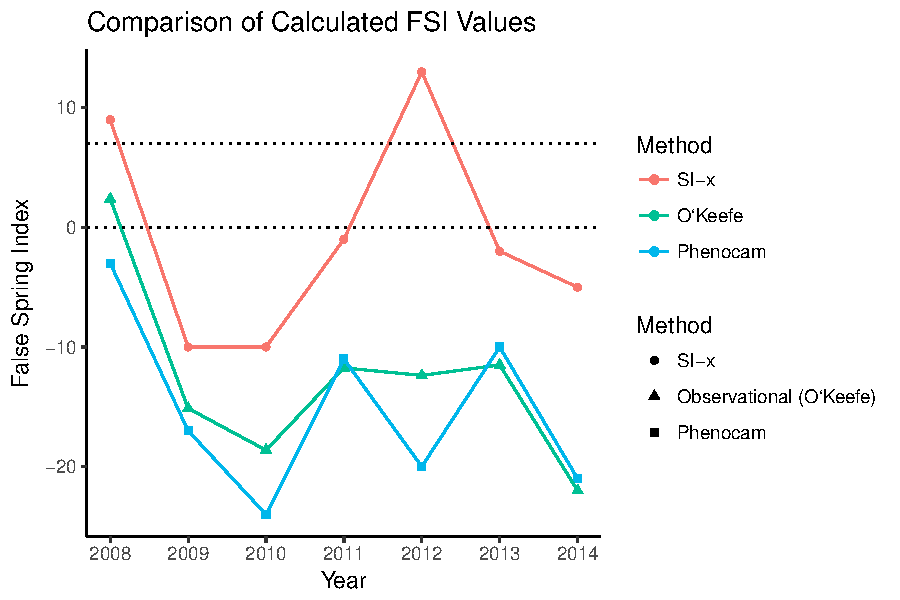
\includegraphics[width=\maxwidth]{figure/fsifig-1} 

}

\caption[False Spring Index (FSI) values from 2008 to 2014 vary across methodologies]{False Spring Index (FSI) values from 2008 to 2014 vary across methodologies. To calculate spring onset, we used the USA-NPN Extended Spring Index tool for the USA-NPN FSI values, which are in red (USA-NPN, 2016), long-term ground observational data for the observed FSI values, which are in green (O'Keefe, 2014), and near-surface remote-sensing canopy data for the PhenoCam FSI values, which are in blue (Richardson, 2015). See supplemental information for extended details. The solid line at FSI=0 indicates a boundary between a likely false spring event or not, with positive numbers indicating a false spring likely occurred and negative numbers indicating a false spring most likely did not occur. The dotted line at FSI=7 indicates the seven-day threshold frequently used in false spring definitions, which suggests years with FSI values greater than seven very likely had false spring events.}\label{fig:fsifig}
\end{figure}



Differing FSI estimated from our three metrics of spring onset for the same site and years highlight variation across functional groups, which FSI work currently ignores --- instead using one metric of spring onset (often from SI-x data, which is widely available) and assuming it applies to the whole community of plants \citep{Allstadt2015, Marino2011, Mehdipoor2017, Peterson2014}. As the risk of a false spring varies across habitats and functional groups \citep{Martin2010} one spring onset date cannot be used as an effective proxy for all species and researchers should more clearly align their study questions and methods. FSI using such estimates as the SI-x may discern large-scale basic trends across space or years, but require validation with ground observations to be applied to any particular location or functional group of species. 

Ideally researchers should first assess the forest demographics and functional groups relevant to their study question, then select the most appropriate method to estimate the date of budburst to determine if a false spring could have occurred. This, however, still ignores variation in the date of leafout (when cold tolerance increases). Further, considering different functional groups is unlikely to be enough for robust predictions in regards to level of damage from a false spring, especially for ecological questions that operate at finer spatial and temporal scales. For many research questions---as we outline below---it will be important to develop false spring metrics that integrate species differences within functional groups, by considering the tolerance and avoidance strategies that species have evolved to mitigate false springs effects. 

\section*{Improving false spring definitions}
\subsection*{Integrating avoidance and tolerance strategies}
While most temperate woody species use cold hardiness to tolerate low winter temperatures, species vary in how they minimize spring freeze damage through two major strategies: tolerance and avoidance. Many temperate forest plants employ various morphological traits to be more frost tolerant. Some species have increased `packability' of leaf primordia in winter buds which may permit more rapid leafout \citep{Edwards2017} and thus shorten the exposure time of less resistant tissues. Other species have young leaves with more trichomes, which protect leaf tissue from herbivory and additionally may act as a buffer against hard or radiative frosts \citep{Agrawal2004, Prozherina2003}. Species living in habitats with drier winters develop shoots and buds with decreased water content, which makes the buds more tolerant to drought and also to false spring events \citep{Beck2007, Kathke2011, Hofmann2015, Morin2007,  Muffler2016, Nielsen2009, Poirier2010}. These morphological strategies are probably only a few of the many ways plants work to avoid certain types of spring frost damage, thus more studies are needed to investigate the interplay between morphological traits and false spring tolerance. 

Rather than being more tolerant of spring freezing temperatures, many species have evolved to avoid frosts by budbursting later in the spring, well past the last frost event. Such species may lose out on early access to resources, but benefit from rarely, if ever, losing tissue to false spring events. They may further benefit from not needing traits related to frost tolerance \citep{Lenz2013}. 

The difference in budburst timing across temperate deciduous woody species---which effectively allows some species to completely avoid false springs---is determined by their responses to three environmental cues that initiate budburst: low winter temperatures (chilling), warm spring temperatures (forcing), and increasing photoperiods \citep{Chuine2010}. The evolution of these three cues and their interactions have permitted temperate plant species to occupy more northern ecological niches \citep{Kollas2014} and decrease the risk of false spring damage for all species \citep{Charrier2011}. Species that budburst late are expected to have high requirements of chilling, forcing and/or photoperiod. For example, the interaction between high chilling and with a spring forcing requirement (that is, a species which requires long periods of cool temperatures to satisfy a chilling requirement before responding to any forcing conditions) will avoid budbursting during periods of warm temperatures too early due to insufficient chilling \citep{Basler2012}. An additional photoperiod requirement for budburst can also allow species to avoid false springs. Species with strong photoperiod cues have limited responses to spring forcing until a critical daylength is met, and thus are unlikely to have large advances in budburst with warming. Thus, as long as the critical daylength is past freeze events, these species will evade false spring events \citep{Basler2014}. 

Given the diverse array of spring freezing defense mechanisms, improved metrics of false spring events would benefit from a greater understanding of avoidance and tolerance strategies across species, especially under a changing climate. If research could build a framework to help classify species into what strategy they employ, estimates of false spring could quickly identify some species that effectively are never at risk of false spring events versus those that more commonly experience false springs. Of this latter group, specific strategies or traits may then help define which species will see the greatest changes in false spring events with climate change. For example, species that currently avoid false springs through high chilling requirements may see the effectiveness of this strategy erode with warming winters \citep{Montwe2018}. Alternatively, for species that tolerate false spring through a rapid budburst to leafout phase, climate change may alter the rate of this phase and thus make some species more or less vulnerable. 

% Cat: I made up some more stuff below in this and the NEXT paragraph, see if it is correct, change as needed and add citations. 
\subsection*{Integrating phenological cues to predict vegetative risk}
Understanding what determines the rate of budburst and the length of time between budburst and leafout is essential for predicting the level of damage from a false spring event. The timing between these phenophases (budburst to leafout), which we refer to as the duration of vegetative risk (Figure \ref{fig:risk}) is a critical area of future research. Currently research shows there is significant variation across species in their durations of vegetative risk, but basic information, such as whether early-budburst species and/or those with fewer morphological traits to avoid freeze damage have shorter durations of vegetative risk compared to other species, is largely unknown but important for improved forecasting. With spring advancing, of species that budburst early those that have shorter durations of vegetative risk may avoid false springs more successfully compared to those that have much longer durations of vegetative risk. This hypothesis, however, assumes the duration of vegetative risk will be constant with climate change, which seems unlikely as both phenophases are shaped by environmental cues. The duration of vegetative risk is therefore best thought of as a species-trait with potentially high variation determined by environmental conditions. Understanding the various physiological and phenological mechanisms that determine budburst and leafout across species will be important for improved metrics of false spring, especially for species- and/or site-specific studies. 

\begin{figure}[H]

{\centering 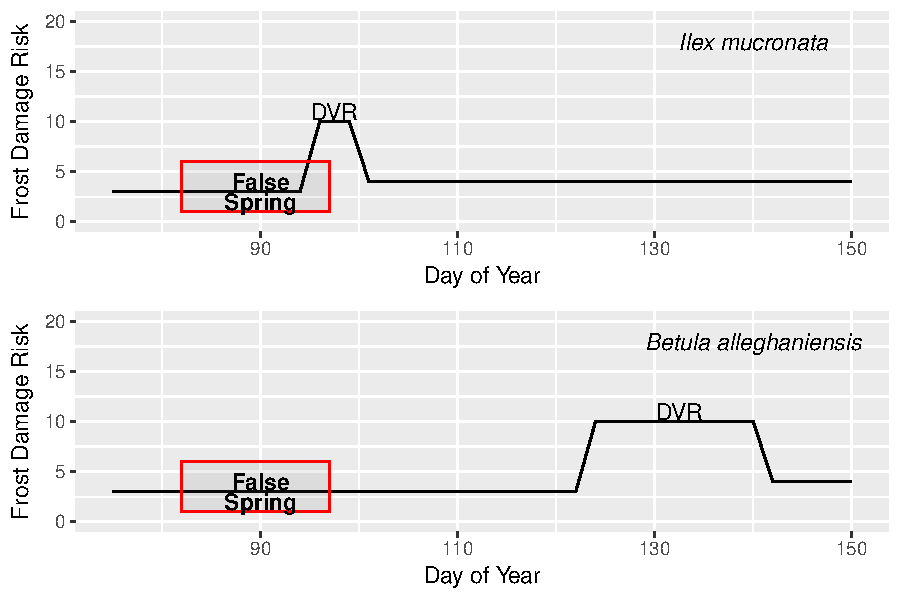
\includegraphics[width=\maxwidth]{figure/risk-1} 

}

\caption{Differences in spring phenology and false spring risk across two species: \textit{Ilex mucronata} (L.) and \textit{Betula alleghaniensis} (Marsh.). We mapped a hypothetical false spring event based on historical weather data and long-term observational phenological data collected at Harvard Forest (O'Keefe, 2014). In this scenario, \textit{Ilex mucronata}, which budbursts early and generally has a short period between budburst (light green squares) and leafout (dark green triangles), would be exposed to a false spring event during its duration of vegetative risk (i.e., from budburst to leafout), whereas \textit{Betula alleghaniensis} would avoid it entirely (even though it has a longer duration of vegetative risk), due to later budburst.}\label{fig:risk}
\end{figure}



Decades of research on phenology provide a starting point to understand how the environment controls the duration of vegetative risk across species. As reviewed above, the three major cues that control budburst \citep[e.g., low winter temperatures, warm spring temperatures, and increasing photoperiods,][]
{Chuine2010} play a dominant role. Comparatively fewer studies have examined all three cues for leafout, but work to date suggests both forcing and photoperiod play major roles \citep{Basler2014, Flynn2018}. The most useful research though would examine both budburst and leafout at once. Instead, most phenological studies currently focus on one phenophase (i.e., budburst or leafout) making it difficult to test how the three phenological cues, and their interactions, affect the duration of vegetative risk.  

With data in hand, phenological cues can provide a major starting point for predicting how climate change will alter the duration of vegetative risk. Robust predictions will require more information, especially the emissions scenario realized over coming decades \citep{IPCC2014}, but some outcomes with warming are more expected than others. For example, higher temperatures are generally expected to increase forcing and decrease chilling in many locations, as well as to trigger budburst at times of the year when daylength is shorter. Using data from a recent study that manipulated all three cues and measured budburst and leafout \citep{Flynn2018} shows that any one of these effects alone can have a large impact on the duration of vegetative risk (Figure \ref{fig:dan}): more forcing shortens it substantially (-15 to -8 days), while shorter photoperiods and less chilling increase it to a lesser extent (+3 to 9 days). Together, however, the expected shifts generally shorten the duration of vegetative risk by 4-13 days, both due to the large effect of forcing and the combined effects of multiple cues. How shortened the risk period is, however, varies strongly by species and highlights how climate change may speed some species through this high risk period, but not others. Additionally, as our results are for a small set of species we expect other species may have more diverse responses, as has already been seen in shifts in phenology with warming \citep{Cleland2006, Fu2015, Xin2016}.

These findings highlight the need for further studies on the interplay among chilling, forcing, and photoperiod cues and the duration of vegetative risk across species. This is especially true for species occupying ecological niches more susceptible to false spring events; even if warming causes a shortened duration of vegetative risk for such species, the related earlier budburst dates could still lead to greater risk of false spring exposure.

% Cat: Can you summarize after the Zohner ref overall what these studies have found? And I think Doug Fir or populus has lots of chilling x coast studies, no?
Studies aiming to predict species shifts across populations (e.g., across a species' range) will also need much more information on how a single species' budburst and leafout timing vary across space. Research to date has studied only a handful of species and yielded no patterns that can be easily extrapolated to other species or functional groups. Some studies have investigated how phenological cues for budburst vary across space, including variation across populations, by using latitudinal gradients \citep{Gauzere2017, Sogaard2008, Way2015, Zohner2016}, which indicates more southern populations tend to rely on photoperiod more than northern populations to better avoid spring frosts. Other studies have examined distance from the coast \citep[see][]{Aitken2015, Harrington2015, Myking2007}, and some have found that distance from the coast is a stronger indicator of budburst timing than latitude \citep{Myking2007}, with populations further inland initiating budburst first, whereas those closer to the coast budburst later in the season. Changes in chilling requirements that impact budburst have been repeatedly documented to vary with distance from the coast, and appear predictable based on local climate variation \citep{Campbell1979, Howe2003}.  
%% Need a space to develop thoughts on what is needed

\begin{figure} [H] 
 \begin{center}
 %\textbf{How Major Cues of Spring Phenology Alter Vegetative Risk}\par\medskip
 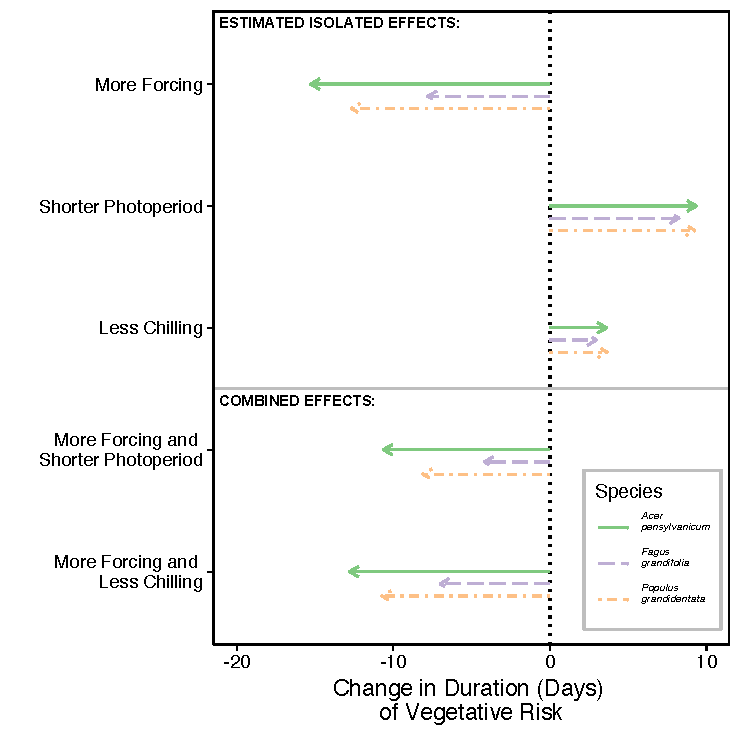
\includegraphics[width=12cm, height=12cm]{..//figure/Exp_plotTPS.pdf} 
 \caption{We examine the effects of phenological cues on the duration of vegetative risk across three species: \textit{Acer pensylvanicum}, \textit{Fagus grandifolia}, and \textit{Populus grandidentata} (see supplemental information for futher details). `More Forcing' is a 5$^{\circ}$C increase in spring warming temperatures, `Shorter Photoperiod' is a 4 hour decrease in photoperiod and `Less Chilling' is a 30 day decrease in over-winter chilling. Along with the estimated isolated effects, we the show the combined predicted shifts in phenological cues with potential climate change (i.e., more forcing with shorter photoperiod and more forcing with less chilling) and the subsequent shifts in duration of vegetative risk across species. To calculate the combined effects, we added the estimated isolated effects of each cue alone with the interaction effects for the relevant cues for each species. }\label{fig:dan} 
 \end{center}
 \end{figure}
% Need to say which treatments.


% show that predictions will require accurate forecasts of the magnitude and direction of how forcing, daylength and chilling will change in the future, as well as how those cues vary across species. 
%Considering the interaction of cues and climate change further complicates understanding species future vulnerabilities to false spring events.  %For example, as climate change progresses, higher spring forcing temperatures may be required for species experiencing insufficient winter chilling (due to warmer winter temperatures), especially at lower latitudes \citep{McCreary1990, Morin2009, Fu2012, Polgar2014, Chuine2010}. 
% Individuals that initiate budburst earlier in the spring may attempt to limit freezing risk by decreasing the duration of vegetative risk in order Further studies are essential 

\subsection* {Integrating predictable regional differences in false spring risk} % Climate, Species Responses risk differences
Understanding the environmental cues that determine the timing and duration of vegetative risk would provide a major step forward in improving metrics of false spring, but then must be combined with an nuanced appreciation of climate. Research to date \citep{Savolainen2007, Vitasse2009, Hanninen2011} highlights the interplay of species cues with a specific location's climate. Climate regime extremes (e.g., seasonal trends, annual minima and annual maxima) vary across regions and are expected to shift dynamically in the future: as climatic regimes are altered by climate change, false spring risk could vary in intensity across regions and time (i.e., regions currently at high risk of false spring damage could become low-risk regions in the future and vice versa). To highlight this, we analyzed five archetypal regions across North America and Europe. Through the use of both phenology \citep{USA-NPN2016, Soudani2012, Schaber2005,  White2009} and climate data \citep[from the NOAA Climate Data Online tool][]{NOAA} we determined the number of false springs (i.e., temperatures at -2.2$^{\circ}$C or below) for each region, which is similar to the FSI approach. We found that some regions experienced harsher winters and greater temperature variability throughout the year (Figure \ref{fig:region} e.g., Maine, USA), and these more variable regions often have a much higher risk of false spring than others (Figure \ref{fig:region} e.g., Lyon, France). (NEED TO EDIT HERE!!) Here, we prove the merit to using FSI work in some studies, such as elucidating the regional differences in false spring risk across population ranges or across different climates. 
% Cat: Do we use FSI to do the above? If so I think we should say it and then point out clearly that these regional differences are a place where simple metrics like FSI may shine a little .... they are designed to pick up such climatic variation (as long as the underlying climate data are robust)!

Understanding and integrating spatiotemporal effects and regional differences when investigating false spring risk---especially for studies at regional or larger spatial scales---would improve predictions as climate change progresses. Such differences depend both on the local climate, the local species and the cues for each species at that location. As we have discussed above, different species within the same location can exhibit different sensitivities to the three cues \citep{Basler2012, Laube2013} so multi-species studies will need to integrate these multiple layers of variation. But single-species studies also must consider layered variation as a single species may have varying cues across space. Based on cues alone then, different regions may have different durations of vegetative risk for the same species \citep {Caffarra2011, Partanen2004, Viheraaarnio2006}, and accurate predictions will need to integrate cue and climatic variation across space.
% CJC (3-Jul-2018): various studies that investigated latitudinal effects indicate that populations growing further north respond to a different interaction of cues than those growing further south. Thus, 
\begin{figure} [H] 
 \begin{center}
 %\textbf{Regional Differences in False Spring Risk}\par\medskip
 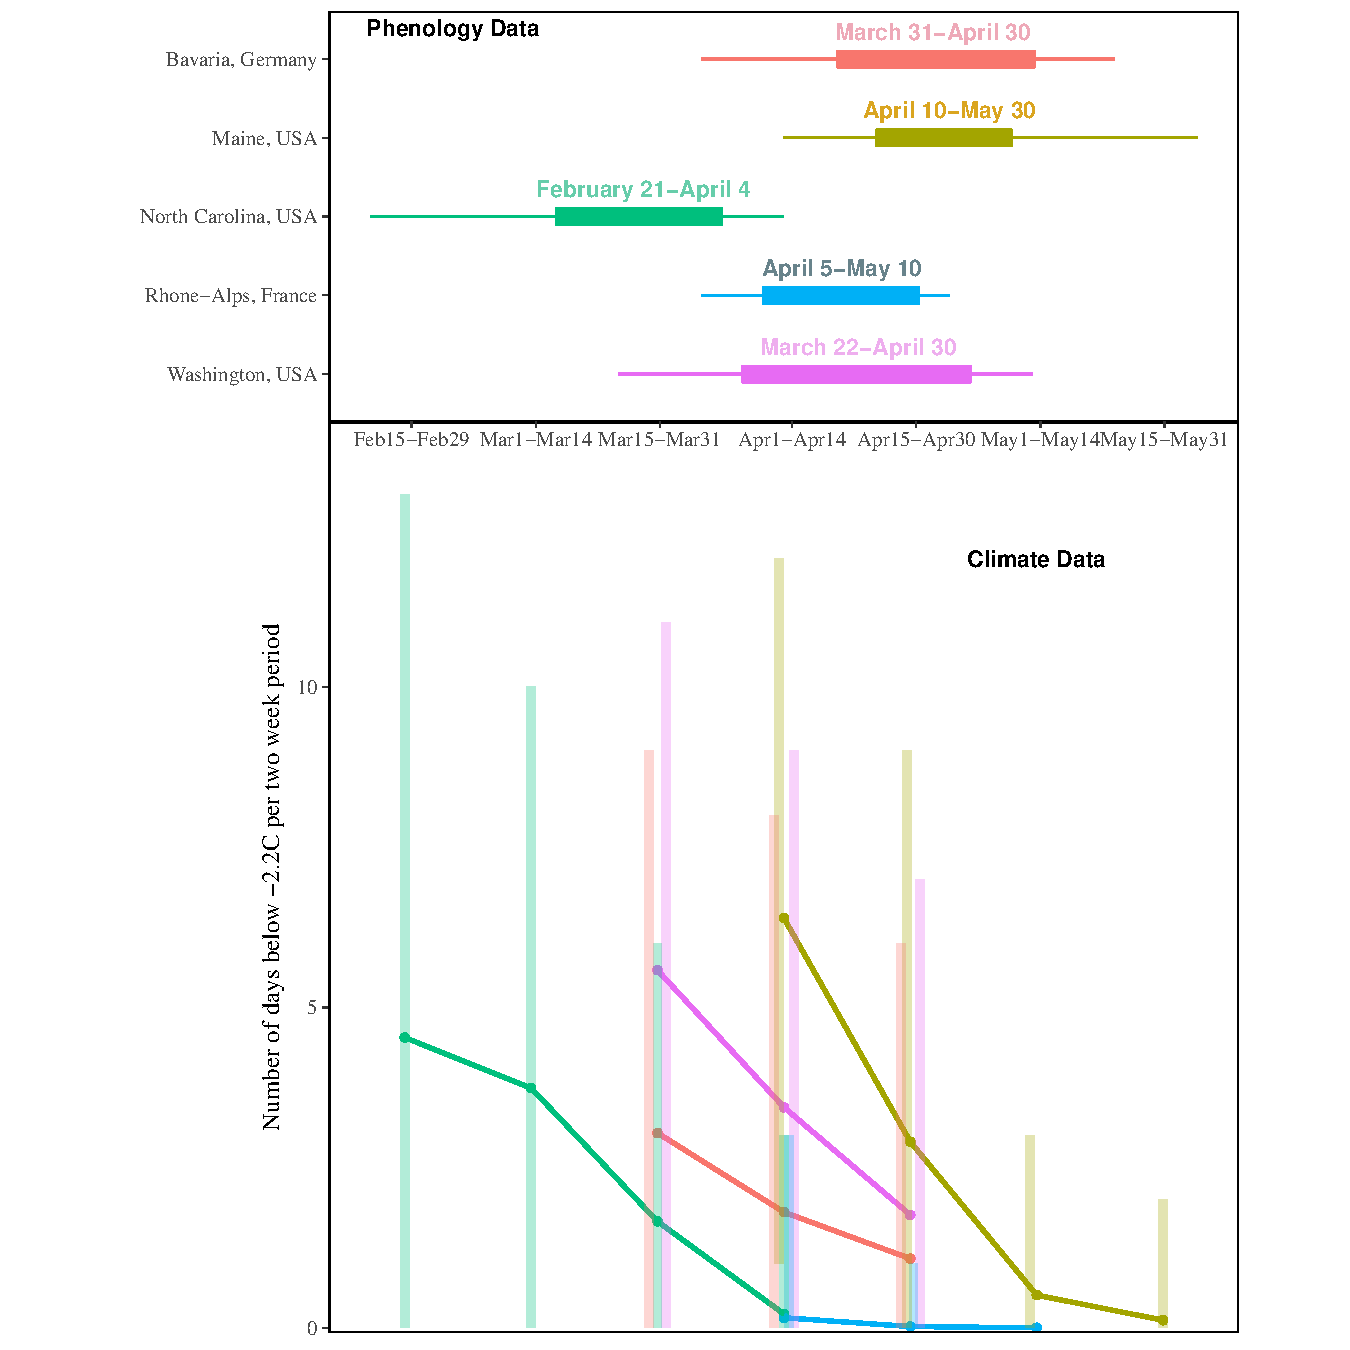
\includegraphics[width=12cm, height=12cm]{..//figure/RegRisk_flipped.pdf} 
 \caption{False spring risk can vary dramatically across regions. Here we show the period when plants are most at risk to tissue loss -- between budburst and leafout (upper, lines represent the range with the thicker line representing the interquartile range) and the variation in the number of freeze days (-2.2$^{\circ}$C) (Schwartz, 1993) that occurred on average over the past 50 years for five different sites (lower, bars represent the range, points represent the mean). Data come from USA-NPN SI-x tool (1981-2016) and observational studies (1950-2016) for phenology (Schaber \& Badeck, 2005; Soudani et al., 2012; USA-NPN, 2016; White et al., 2009) and NOAA Climate Data Online tool for climate (from 1950-2016). See supplemental information for futher details on methods. } \label{fig:region}  
 \end{center}
 \end{figure}


\section*{The future of false spring research}
% Cat: I made lots of changes here to better address reviewer concerns and build on what we outlined above, see what you think. 
With climate change, more researchers across diverse fields and perspectives are studying false springs. Simplified metrics, such as the FSI, have helped to understand how climate change may alter false springs now and in the future. They have helped estimate potential damage and, when combined with methods that can document tissue loss \citep[e.g., PhenoCam images can capture initial greenup, defoliation due to frost or herbivory, then refoliation,][]{Richardson2018b} have helped document the prevalence of changes to date. Related work has shown that duration of vegetative risk can be extended if a freezing event occurs during the phenophases between budburst and full leafout \citep{Augspurger2009}, which could result in exposure to multiple frost events in one season. Altogether they have provided an important way to meld phenology and climate data to understand impacts on plant growth and advance the field (CITES). As research in this area grows, however, the use of simple metrics to estimate when and where plants experience damage may slow progress in many fields. 

% Cat: Be careful with defining native; your original text defined lilac as non-native, but that is only true for certain locations!
As we have outlined above, current false spring metrics depend on the phenological data used, and thus often ignore important variation across functional groups, species, populations, and life-stages---variation that is critical for many types of studies. Many studies in particular use gridded spring-onset data, such as those available through SI-x. Studies aiming to forecast false spring risk across a species' range using SI-x data may do well for species similar to lilac (\emph{Syringa vulgaris}), such as other closely related shrub species distributed across or near lilac's native southwestern European range. But we expect predictions would be poor for less similar species. No matter the species, current metrics ignore variation in cues underlying the duration of vegetative risk across space (and, relatedly, climate) and assume a single threshold temperature and 7-day window. These deficiencies, however, highlight the simple ways that metrics, such as FSI can be adapted for improved predictions. For example, researchers interested in false spring risk across a species range can gather data on freezing tolerance, the environmental cues that drive the variation in the duration of vegetative risk and whether those cues vary across populations, then adjust the FSI or similar metrics. Indeed, given the growing use of the SI-x for false spring estimates research into the temperate thresholds and cues for budburst and leafout timing of \emph{Syringa vulgaris} could refine FSI estimates using SI-x. 

Related to range studies, studies of plant life history will benefit from more specialized metrics of false spring. Any estimates of fitness consequences of false springs at the individual- population- or species-levels must integrate over important species, population and life-stage variation. In such cases, careful field observational and lab experimental data will be key. Through such data, researchers can capture the variations in temperature thresholds, species- and lifestage-specific tolerance and avoidance strategies and climatic effects, and more accurately measure the level of damage.  

Though time-consuming we suggest research to discover species \(x\) life-stage specific freezing tolerances and related cues determining the duration of vegetative risk has the greatest opportunity to make major advances in fundamental and applied science. Such studies can help determine at which life stages false springs have important fitness consequences, and whether tissue damage from frost for some species \(x\) life stages actually scales up to minimal fitness effects. As more data are gathered, researchers can test whether there are predictable patterns across functional groups, clades, life history strategies, or related morphological traits. Further, such work would form the basis to predict how future plant communities may be reshaped by changes in false spring events with climate change. False spring events could have large scale consequences on forest recruitment, and potentially impact juvenile growth and forest diversity, but predicting this is another research area that requires far more and improved species-specific data. 

% Need more cites here of general papers on ecosystem models. 
While we suggest most studies at the individual to community levels need far more complex metrics of false spring to make major progress, simple metrics of false spring may be appropriate for a suite of studies at ecosystem-level scales. Single-metric approaches, such as the FSI, are better than not including spring frost risk in relevant studies. Thus, these metrics could help improve many ecosystem models, including land surface models (CITES). In such models, the SI-x would provide researchers with predicted shifts in frequency of false springs under emission scenarios. The Ecosystem Demography (ED) model already integrates phenology data by functional group \citep{Kim2015, Moorcroft2001}, by adding last freeze date information, FSI could then be evaluated to predict false spring occurrence with predicted shifts in climate. By including even a simple proxy for false spring risk, the ED model, and similar models, could better inform predicted range shifts. As such models often form a piece of global climate models (CITES), incorporating false spring metrics could refine estimates of future carbon budgets and related shifts in climate. As more data helps refine our understanding of false spring damage for different functional groups, species and populations, these new insights can in turn help improve false spring metrics used for ecosystem models. Eventually earth system models could include feedbacks between how climate shifts alter false spring events, which may reshape forest demography, and in turn alter the climate itself.  

%At the next level, models such as PHENOFIT, incorporate abiotic stresses to assess predicted range shifts \citep{Gritti2013, Chuine2001b}
% \section*{Conclusion} % I personally don't think we need this any more given the new ending section ... I took some of the text to make the abstract better match the current draft of the paper. 

\section*{Acknowledgments}
We thank D. Buonaiuto,  W. Daly, A. Ettinger, and I. Morales-Castilla for comments and insights that improved the manuscript. 

\nocite{Schwartz1993}
\nocite{Barker2005}
\nocite{Sanchez2013}
\nocite{Longstroth2012}
\nocite{Barlow2015}
\nocite{Longstroth2013}
\nocite{Charrier2011}
\bibliography{..//refs/SpringFreeze.bib}

\end{document}
